\chapter{Theoretical background}
\label{ch:theoretical-background}

In this chapter, we shall describe the theoretical background
taken under consideration for the developed models and analysis, including
the prevalence estimation problem (Section
\ref{sec:prevalence_estimation_problem}), Respondent-driven sampling (Section
\ref{sec:respodent_driven_sampling}), Bayesian statistics (Section
\ref{sec:bayesian_statistics}), and computational methods (Section
\ref{sec:computational_methods}) used in our research.

\section{Prevalence estimation problem}
\label{sec:prevalence_estimation_problem}

The study of how health-related conditions are distributed among populations
is known as {\em Epidemiology} \cite[p. 32]{rothman2008modern}, which aims to derive valid estimates for
potential causes from diseases that affect people. It is a fundamental
research area in policy formulation, implementation of prevention programs,
and development of laws. In order to accomplish these goals, the
epidemiologists use some {\em measures of disease frequency}, including {\em
incidence} and {\em prevalence}. The former is related to the proportion of
new cases of a disease given a period of time, while the latter is the proportion
of individuals exposed at time $t$ and it is the object of
study of this section. An interesting point is the following:

\begin{citacao}
  Diseases with high incidence rates may have low prevalence if they are rapidly fatal or quickly cured. Conversely, diseases with very low incidence
  rates may have substantial prevalence if they are nonfatal but incurable.
  \cite[p. 46]{rothman2008modern}.
\end{citacao}

As a result, prevalence represents both incidence and the duration of disease. \textcite[p. c18]{noordzij2010measures} highlights that
prevalence reveals the burden of a disease in respect to its effects on
society, such as, monetary costs, quality of live, and morbidity. They also
comment that when measured periodically, its evolution can identify potential
causes of the infection and prevention and care methods. We remark that when it is impossible to test every individual at the same
time, we assume that all individuals remain exposed to the disease at time of
the last tested individual.

Consider a population of interest and a known condition, such as, for instance,
a disease or a binary behavior. A diagnostic test is done in the individuals
to measure the presence or the absence of this condition, such as serological
tests. Mathematically, we denote $\theta \in (0,1)$ the prevalence of the
condition, which is the parameter of interest. Let $I$ be a index set for the
individuals. We also denote $Y^{\mathrm{true}}_i$ the indicator function of
the presence of the condition in the i$^{th}$ individual, that is, 
$$Y^{\mathrm{true}}_i = \begin{cases}
  1, &\text{if individual } i \text{ has the condition.} \\
  0, &\text{otherwise.}
\end{cases}$$

Assume for simplicity that all tests are performed at time $t$. Assume that
$Y_i$ indicates the result of the test, then 
$$Y_i = \begin{cases}
  1, &\text{if test was positive in individual } i. \\
  0, &\text{otherwise.}
\end{cases}$$

Since it is not usually feasible to test everyone in the population, it is
necessary to random select individuals from the population. On that point,
other sampling approaches may be better options, such as stratified random
sampling, systematic sampling, and two-stage cluster sampling. From that
experiment, we get a sample $y = \{y_1, ..., y_n\}$. Based on that outcomes the Maximum Likelihood Estimator is the following expression 
\begin{equation}
    \label{eq:naive-estimator}
    \hat{p} = \frac{1}{n}\sum_{i=1}^n y_i, 
\end{equation}
which is an estimator for the {\em apparent prevalence}, that is, the
probability of a positive outcome. 

However, this estimator assumes that the diagnostic test used is perfect,
which is often incorrect \todo{Provide some reference}. It is also not
interesting when the samples are not randomly selected (See Section
\ref{sec:respodent_driven_sampling}). From that point, it is crucial to regard
the evaluation of the diagnostic procedure by some measurement. \textcite[p.
2]{vsimundic2009measures} presents several options with different aspects,
such as the {\em likelihood ratio}, {\em sensitivity and specificity}, and
{\em the area under the ROC curve}. In this work, we consider the sensitivity
and specificity of the test.

A perfect test would discriminate every sick individual from the non-sick ones.
Given that there is not such thing, we suppose having a {\em gold standard
test} that is the best available test \cite{versi1992gold} to diagnose a
particular disease. Its result is a proxy for the real $Y^{\mathrm{true}}_i$ and 

\begin{citacao}
  In the context of infectious diseases, a gold standard can be a very precise
  molecular test that detects the presence of the pathogen’s genetic material,
  polymerase chain reaction (PCR) for instance. \cite[p. 125]{bastos2021modelling}.
\end{citacao}

From the gold standard, we can evaluate a second test, typically faster or
cheaper. The possible results upon comparing these tests are presented in
table \ref{table:two-by-two}. The definitions for each initials in the table
are the following: 

\begin{alineas}
  \item true positive (TP): when both tests agree that the individual has the
  disease;
  \item true negative (TN): when both tests agree that the individual does not
  have the disease;
  \item false positive (FP): when the test under evaluation has a positive
  diagnose, despite the golden standard being negative;
  \item false negative (FN): when the test under evaluation has a negative
  diagnose, despite the golden standard being positive.
\end{alineas}

\begin{quadro}[!ht]
  \centering
  \caption[Chart]{Two-by-two table that compares the result from the gold standard to
  the test under evaluation.}
  \begin{tabular}{c|c|c|}
  \cline{2-3}
                                               & $Y = 0$ & $Y = 1$ \\ \hline
  \multicolumn{1}{|c|}{$Y^{\mathrm{true}}= 0$} & TN    & FP    \\ \hline
  \multicolumn{1}{|c|}{ $Y^{\mathrm{true}}= 1$} & FN    & TP    \\ \hline
  \end{tabular}
  \fonte{Prepared by the author (2021) and based on \textcite[p. 126]{bastos2021modelling}.}
  \label{table:two-by-two}
\end{quadro}

\begin{remark}
  When a gold standard test is not available, which is called {\em no gold standard
  situations} \cite[p. 1]{rutjes2007evaluation}, other methods should be
  considered such as the construction of reference standard by giving the
  patients either different or the same tests and combining the results
  somehow. For more details, \textcite{rutjes2007evaluation} does a literature
 review on the topic.  
\end{remark}

For now, we drop the index $i$ in the random variables $Y_i$ and
$Y_i^{\mathrm{true}}$. Let $p = \Pr(Y = 1)$ be the probability of a positive test.
We call $p$ the {\em apparent prevalence} since it is what the researchers 
observe. Equation \eqref{eq:naive-estimator} is an estimator for it. 
We also have that $\Pr(Y^{\mathrm{true}} = 1) = \theta$. Notice that $p$
depends on the used test, while $\theta$ does not. In prevalence estimates, we 
will only have $\theta = p$ if the test is perfect or the test is the 
gold standard itself. Define the following: 

\begin{definition}[Sensitivity]
  Probability of a positive test correctly identified. In mathematical terms,
  conditioned on $Y^{\mathrm{true}} = 1$, the {\em sensitivity} $\gamma_s$ is 
  the probability of $Y = 1$: 
  \begin{equation}
    \gamma_s = \Pr(Y = 1|Y^{\mathrm{true}} = 1). 
  \end{equation} 
\end{definition}

\begin{definition}[Specificity]
  Probability of a negative test correctly identified. In mathematical terms,
  conditioned on $Y^{\mathrm{true}} = 0$, the {\em specificity} $\gamma_e$ is 
  the probability of $Y = 0$: 
  \begin{equation}
    \gamma_e = \Pr(Y = 0|Y^{\mathrm{true}} = 0). 
  \end{equation} 
\end{definition}

\begin{theorem}[Relation between prevalence and apparent prevalence] These quantities are related by the following equation:
  \begin{equation}
    \label{eq:apparent-true-prevalence}
    p = \gamma_s\theta + (1-\gamma_e)(1-\theta).
  \end{equation}
  
\end{theorem}

\begin{proof}
  This is a direct application of the definition of conditional probability
  and the countable additivity axiom of Probability:
  \begin{equation*}
    \begin{split}
      p &= \Pr(Y = 1) = \Pr(Y = 1, Y^{\mathrm{true}} = 1) + \Pr(Y = 1, Y^{\mathrm{true}} = 0) \\
      &= \Pr(Y=1|Y^{\mathrm{true}}=1)\Pr(Y^{\mathrm{true}}=1) + \Pr(Y=1|Y^{\mathrm{true}}=0)\Pr(Y^{\mathrm{true}}=0) \\
      &= \Pr(Y=1|Y^{\mathrm{true}}=1)\Pr(Y^{\mathrm{true}}=1) \\ 
      &+ (1 - \Pr(Y=0|Y^{\mathrm{true}}=0))(1-\Pr(Y^{\mathrm{true}}=1)) \\
      &= \gamma_s\theta + (1 - \gamma_e)(1-\theta).
    \end{split}
  \end{equation*} 
\end{proof}

The intuition behind this equation is pretty simple: the proportion
of positive test counts the correct identified exposed individuals and the
incorrect identified not exposed. Equation \eqref{eq:apparent-true-prevalence}
also reveals that if $\gamma_s = \gamma_e = 1$, we have the trivial 
case $p = \theta$. Moreover, if $\gamma_s = \gamma_e = 0.5$, we have that
$p = 0.5$ and there is no information about $\theta$. 

A frequentist approach assumes that $\theta$ is fixed and unknown. Its
inference is based on the point 
estimate for the apparent prevalence $\hat{p}$ given in Equation
\eqref{eq:naive-estimator}, along with a Confidence Interval, such as the Wald
Confidence Interval built with a normal approximation. In order to provide a 
point estimate for $\hat{\theta}$, \textcite[p. 73]{rogan1978estimating}
propose
\begin{equation}
  \label{eq:rogan-estimate-prevalence}
  \hat{\theta}^{RG} = \frac{\hat{p} - (1-\gamma_e)}{\gamma_s + \gamma_e -
1}.
\end{equation}
Suppose a disease with prevalence $\theta = 0.01$. In this case, we would have
that $p \approx 1 - \gamma_e$ by equation \eqref{eq:apparent-true-prevalence}.
Given the randomness, it is possible to have $\hat{p} < 1 - \gamma_e$, which
would define a useless estimative for $\theta$. Besides that, Confidence Intervals for that 
expression does not include uncertainty about $\gamma_e$ and $\gamma_s$. On
the other side, a Bayesian approach let $\theta$ be a random variable,
allowing the researcher to incorporate their uncertainty on the prior
distribution, which is explained in Section
\ref{sec:bayesian_statistics}. It also allows to include uncertainty in
sensitivity and specificity of the test. According to \textcite{branscum2005estimation}:
\begin{citacao}
  Diagnostic-test evaluation is particularly suited to the
  Bayesian framework because prior scientific information about the
  sensitivities and specificities of the tests and prior information about the prevalences of the sampled
  populations can be incorporated. \cite[p. 1]{branscum2005estimation}.
\end{citacao}

Therefore, this work focus on the Bayesian paradigm. 

\subsection{Correlation between sensitivity and specificity}
\label{sec:correlation-sensitivity-specificity}

A general method for a diagnostic or screening test is to construct a
continuous scale measuring some related quantity to the disease and to define
a cut-off number, such that values higher than the threshold indicate the
presence of the illness. Suppose the cut-off is high, almost the maximum value
of the scale. Therefore, the majority of the population will be tested
negative. There will be a lot of false-negative individuals but a few
false-positive ones, which implies that sensitivity is low and specificity is
high. If the threshold is smaller, the opposite effect happens. Nonetheless,
sensitivity and specificity are negatively correlated. \textcite[p.
46]{parikh2008understanding} gives a more practical example. Observe that this
correlation is related to the estimation of the parameters, then it can only
be noticed in meta-analysis studies. 

\section{Respondent-driven sampling}
\label{sec:respodent_driven_sampling}

Respondent-driven sampling (RDS) is a procedure developed by Heckathorn
\cite[]{heckathorn1997} to survey {\em hidden} or {\em hard-to-reach
populations}, whose main characteristic is the absence of a sampling frame,
i.e.,it is not possible to enumerate its individuals since size and boundaries
are unknown. The second characteristic of these populations is the
confidentiality concerns, given that membership is stigmatized or illegal.
With that aspect, traditional sampling methods which produce probability
samples are infeasible. To overcome this, Snowball Sampling \cite[]{goodman1961}
is the most common method, and it relies on the respondents to nominate more 
subjects within the population as a snowball. Examples of studied groups
include people who inject drugs (PWID), men who have sex with men (MSM), and
female sex workers (FSW) \cite[p. 66]{gile2018methods}. 

Heckathorn's proposal \citeyear{heckathorn1997} was to specialize this method without the need of
nominating peers. In this approach, the researchers select some individuals,
called {\em seeds} from the target population, and give them a fixed amount of
{\em recruitment coupons} to recruit their peers. Each recipient of the coupons
reclaims it in the study site, is interviewed, and receives more coupons to
continue the recruitment. This process occurs until it reaches some stopping
criteria, such as the sample size achieving some desired number. The sampling
is without replacement, so the participants cannot be recruited more than
once. Moreover, the respondents inform how many subjects from the population
they know. Other less usual methods include Key Important Sampling \cite{deaux-callaghan1985}, 
and Targeted Sampling \cite{watters-biernacki1989}, both are convenience
sampling methods. 

According to \textcite[p. 66]{gile2018methods}, there are two main advantages
of RDS over other snowball samplings. First, the fixed number of recruitment
coupons enforces the network gets deeper and distant from the seeds, which
reduces the dependence of the final sample from the initial chosen by
researchers. Second, since the recruited subjects do not have to name their
peers, confidentiality is maintained until the recruitment is completed.
Other problems cited by \textcite[p. 175]{heckathorn1997} include biases
towards individuals who are more cooperative, biases by masking when the
participants do not name friends for the next wave to protect them, and
individuals with more links may be oversampled. RDS offers a solution with a
{\em dual incentive system}, explained in Subsection
\ref{sec:sampling-procedure}. 

Since the creation of the method by Heckathorn, several papers have been
published, as \autoref{fig:chart-research-rds} presents. The figure was produced searching
publications with the term ``Respondent-driven sampling.'' These works generally
aim to give basis to public health policies. Good examples in Brazil are
\cite{damacena2019application}, \cite{mota2012respondent}, and
\cite{bastos2018hiv}. \textcite{damacena2019application} apply the RDS method
to carry out biological and behavioral surveillance in FSW populations from twelve cities
in Brazil. \textcite{mota2012respondent} proposes the RDS method in MSM populations from ten cities in
Brazil. \textcite{bastos2018hiv} study several sexually transmitted infections among
transgender women from twelve Brazilian cities.  

\begin{figure}
  \centering  
  \caption{\label{fig:chart-research-rds}Publications by year with the term
  ``Respondent driven sampling'' from 1997 to 2021.}
  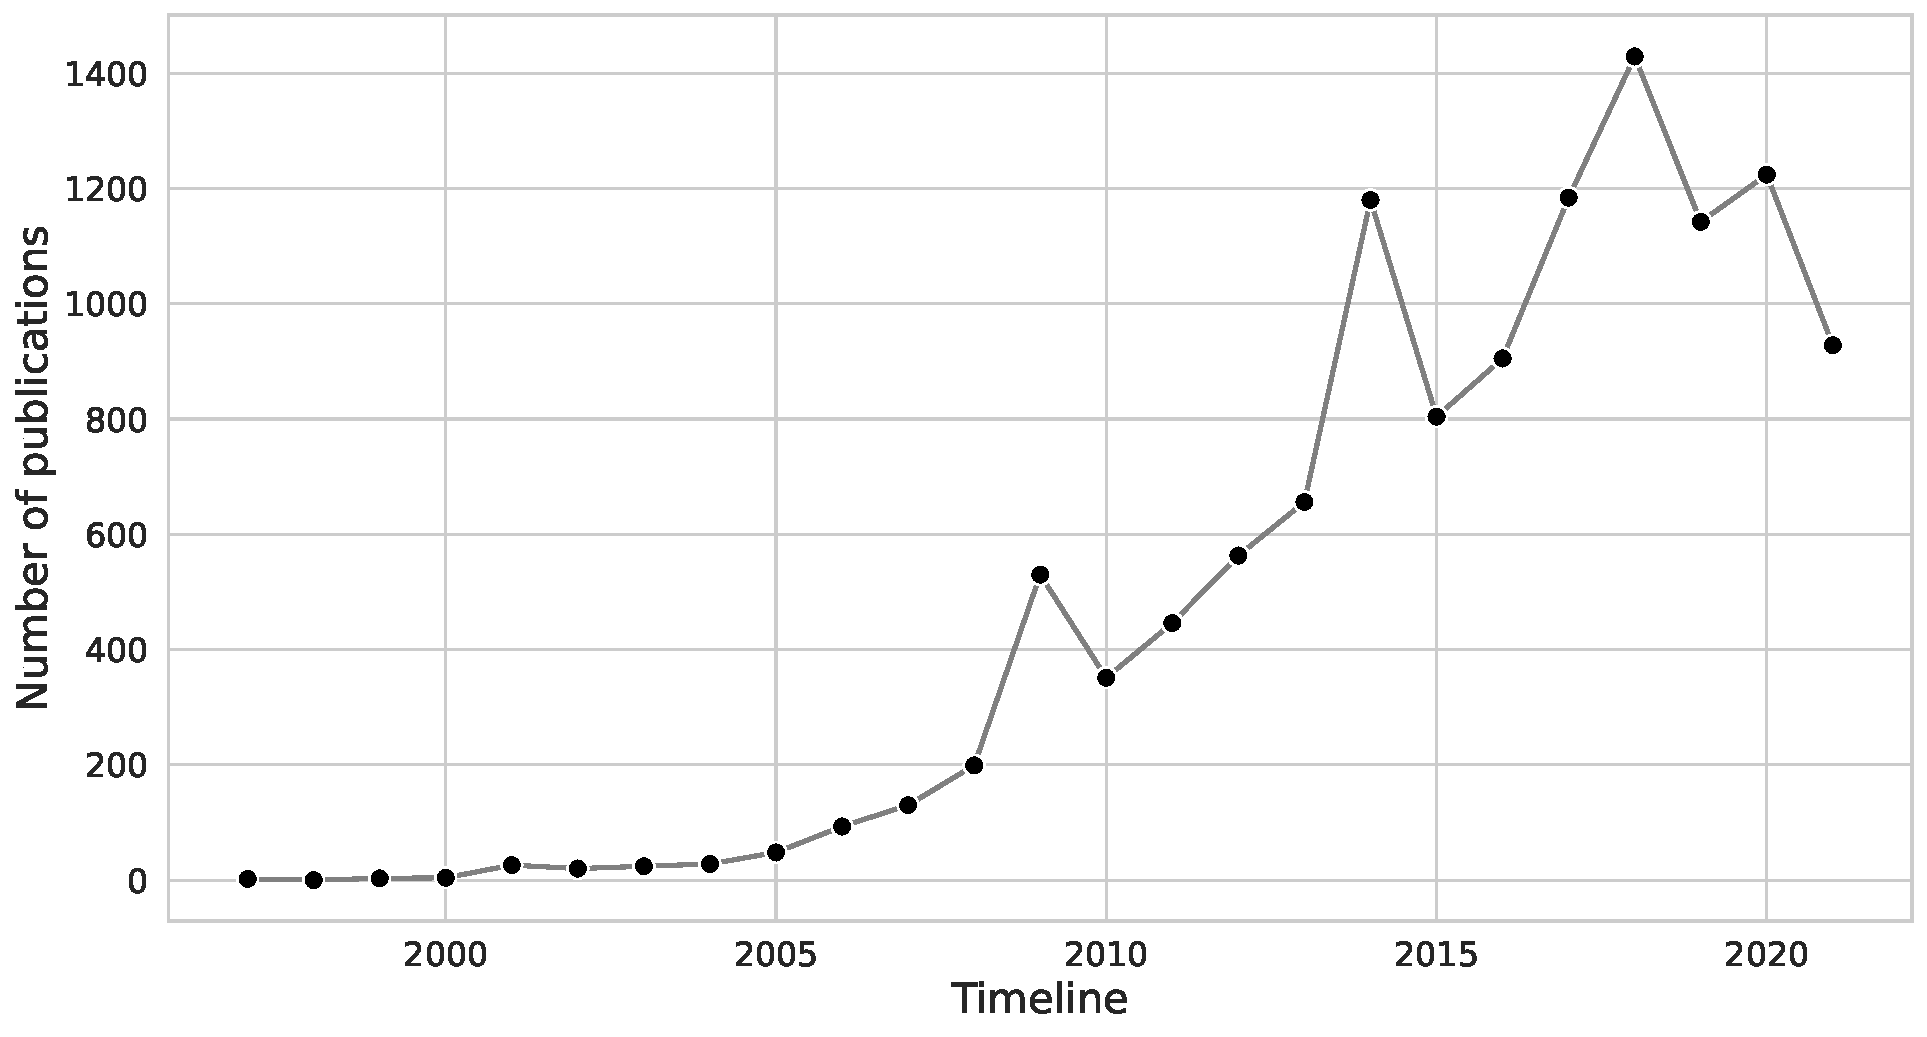
\includegraphics[width=14cm]{chart_research_growing_rds.pdf}
  \fonte{htpps://app.dimensions.ai. Exported on October 31, 2021.}
\end{figure}

\subsection{Details about the sampling procedure}
\label{sec:sampling-procedure}

The RDS method was expanded by \textcite{heckathorn2002}. It detailed two aspects: 
introducing a way to correct {\em homophily} biases that is the tendency for
individuals to connect to others similar to them, and {\em personal network size} or
{\em degree} that is the number of connections of an individual within the
target population. It also presented a bootstrapping procedure to quantify
uncertainty about inferences. \textcite{salganik2004sampling} slightly modified the
RDS procedure and introduced proof that under some regularity conditions, RDS
estimators were asymptotically unbiased. \textcite{world2013introduction}
is a reference to know how to execute an RDS survey. According to it: 

\begin{citacao}
  Seeds are non-randomly selected members of the survey population who initiate the RDS
  recruitment process. From each seed, a recruitment chain is expected to grow. Seeds play
  an extremely important role in conducting an RDS survey. \cite[p. 70]{world2013introduction}.
\end{citacao}

No rule was established on the number of seeds to start the sampling. It
typically varies from 2 to 32, with the mean being 10 \cite[p. 70]{world2013introduction}. The number can not be
small since unsuccessful recruitments are common. A diverse choice among the
target population may accelerate the convergence to equilibrium. It also
allows the access to isolate and subpopulations. After this selection, three
coupons are distributed to each participant. The coupons musta have
information about survey site location, an unique identification code,
telephone number, and opening hours. \textcite[p. 67]{gile2018methods}
highlights that ``this number is chosen to strike a balance between the
inferencial desire [...] and the practical necessity of guarding against early
termination of the sample trees.'' 

Subjects receive a reward for being interviewed and recruiting their peers
within the target population, which establishes a dual incentive system. The
{\em primary incentive} is the {\em individual-sanction-based control}, so there is a
reward for participating in the survey. The second one is the {\em
group-mediated social control} that influences the participants to induce
others to comply to get the remuneration for the recruitment. When social
approval is relevant for the members, recruitment can be more efficient and
cheaper. It happens because material incentives are converted into peer-based symbolic since there is
social influence involved. In conclusion, consenting to be recruited provide
material and symbolic motivation to both recruiter and participant. 

For an illustrative example, \autoref{fig:rds-example-drug-users} presents a recruitment structure
based on a respondent-driven sample among 303 heavy drug users from
Curitiba collected between July 28, 2008, and October 18, 2009  
\cite[Web Appendix]{salganik2011assessing}. Five seeds were chosen within the
population, the fifth being a month after the other four since the fourth seed was
unsuccessful. Each participant received three coupons and the mean number of
recruited individuals per recruiter was around 0.98. 

\begin{figure}
  \centering
  \caption{\label{fig:rds-example-drug-users}RDS structure among heavy drug users
  in Curitiba.}
  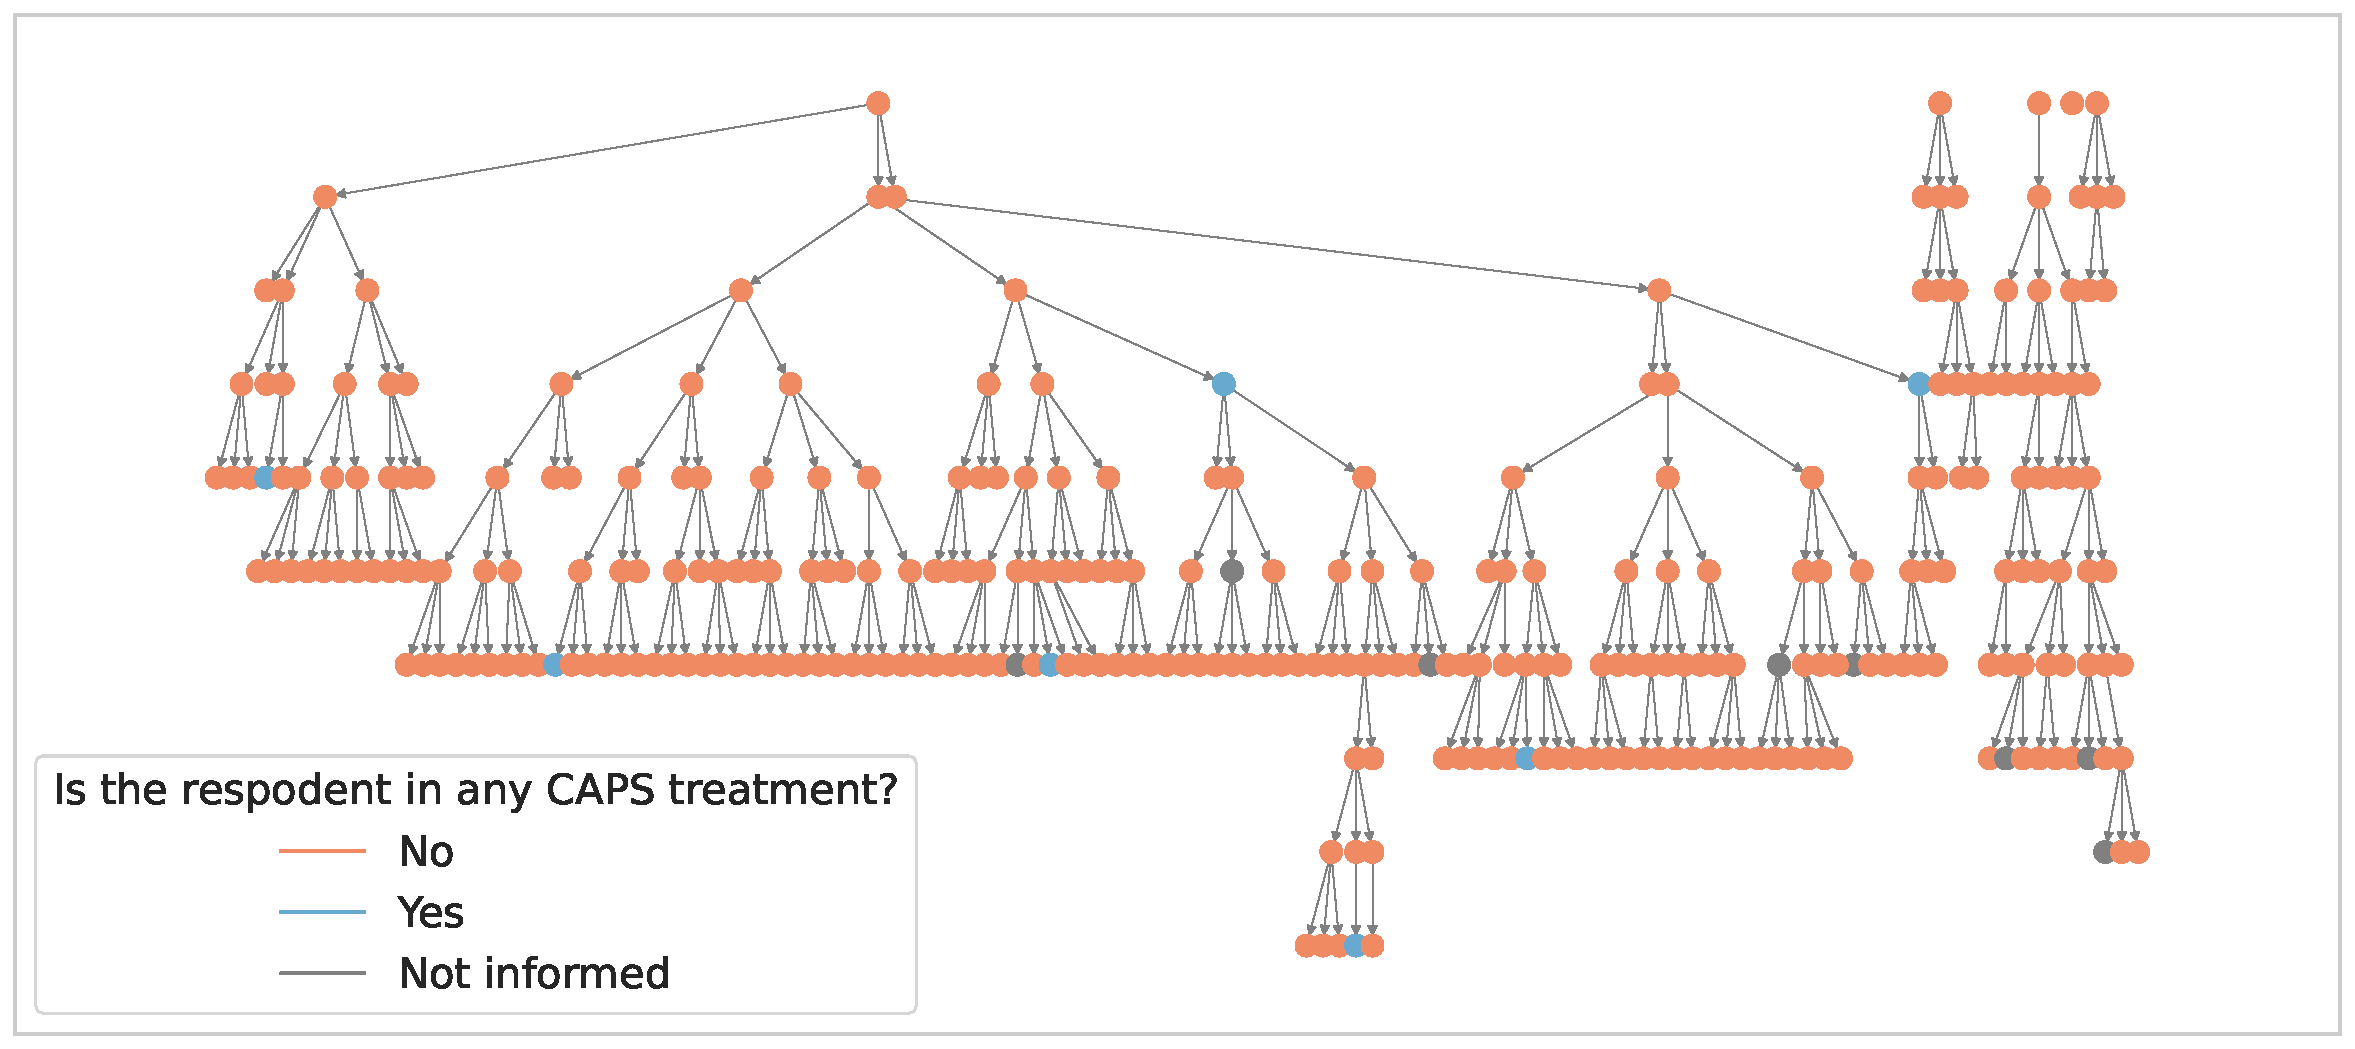
\includegraphics[width=145mm]{rds_example_drug_users.pdf}
  \fonte{Data extracted from \cite{salganik2011assessing} and figure prepared
  by the author (2021). The respondents were asked whether they are in any ``Centro de
  Atenção Psicossocial (CAPS)'' (Psychosocial Care Center) treatment program
  for drug use. }
\end{figure}

\subsection{Assumptions and statistical properties}

RDS is a successful recruitment method for reaching hard-to-reach populations
since the respondents recruit most of the participants. On the other hand,
this characteristic also makes it hard to derive statistical properties
without making strong assumptions of the recruitment process.  Some hypotheses
are related to specific models, which are presented in Section
\ref{sec:models-rds-process}:   

\begin{alineas}
  \item sampling is not uniformly random among the individuals since some have more
  connections than others, which gives them a higher probability of being
  recruited. Those with more contacts should reduce the weighting in the
  inferences, but this also relies on another assumption: self-reported degree
  should be accurately measured \cite[p. 297]{gile2010respondent};
  
  \item \label{item:without-replacement} recruitment is without replacement, given that respondents are not
  allowed to participate more than once. It compromises inferences since the
  probability of inclusion in the survey also depends on the number of
  individuals participating until the recruitment time \cite[p.
  299]{gile2010respondent}. To derive an RDS estimator, 
  \textcite[p. 81]{volz2008probability} requires a small sampling fraction to
  compensate for breaking this assumption;

  \item {\em homophily} is the tendency of individuals to connect within the same
  group. For instance, men tend to recruit more men to women. If the process
  has zero homophily, it indicates that individuals do not regard the group to
  recruit. On the other hand, if homophily is one, all the connections are
  intragroup \cite[p. 20]{heckathorn2002}. \textcite[p. 21]{heckathorn2002} proved
  that under certain conditions (see Subsection \ref{sec:models-rds-process}),
  the respondent-driven sample is unbiased with respect to homophily if it is
  equal for each group;

  \item the connections generated by the RDS process  \autoref{item:without-replacement}violate the independence 
  between the samples through {\em clustering}, i.e., people are more likely 
  to connect to those similar \cite[p. 14]{avery2021statistical};
  
  \item respondent-driven sampling produces a branching structure that makes
  it impossible to observe links between two people who don't recruit each
  other \cite[p. 17]{gile2015network}. It constitutes a missing data problem, according to \textcite[p.
  190]{crawford2016};

  \item in apparent contraction to \autoref{item:without-replacement}, to
  the distribution achieve its convergence and remove the biases induced by
  the initial sample, enough waves of recruitments are necessary \cite[p. 186]{heckathorn1997};
  
  \item \textcite[p. 2225]{goel2009respondent} defines {\em bottleneck}
  as the probability of cross-group recruitment. It happens when the
  recruitment chain remains inside an identified subgroup of individuals. In that
  situation, ``studies should be conducted separately within each tier.''
  \cite[p. 75]{gile2018methods}. As an expository example,
  \textcite[p. S139]{toledo2011putting} observes strong geographical
  heterogeneity among a population of heavy drug users in Rio de Janeiro. 
\end{alineas}

\subsection{Models for the RDS Process}
\label{sec:models-rds-process}

Since its inception, several authors have tried to better understand and model
the RDS process because of its non-probability nature. Each modelling approach
aims to approximate even more the network structure to yield more reliable
inferences. In this section, we present some of them. Let $G = (V,E)$ be an
undirected graph representing the hidden population, such that $|V| = N$, and
$A \in \{0,1\}^{N \times N}$ its adjacency matrix, where $A_{ij} = 1$ if there
is a connection between individuals $i$ and $j$, and $A_{ij} = 0$ otherwise.
We denote $|V|$ to mean the number of nodes, and $|E|$ the number of edges in
the graph $G$. The choice of an undirected model for the hidden population is very common,
but not obliged. The degree of a person is, therefore, $d_i = \sum_{j=1}^N
A_{ij}$.\todo{Include notation of RDS used posteriorly.} 

Besides the following models, there are two additional and relevant works  to
cite. \textcite{goel2009respondent} described RDS as a Markov chain Monte
Carlo to analyse the structure created by the recruitment links. They deeply
discussed the problems that bottlenecks can cause.
\textcite{mclaughlin2021bayesian} developes a Bayesian model for the
recruitment process considering preferential selection based on the covariates.


\subsubsection{First-order Markov process}
\label{sec:first-order-markov-process}

This approximation was the first model proposed by \textcite{heckathorn1997}. 
He argues RDS recruitment has the characteristic that ``any subject's recruits are
a function of his or her type, such as his or her ethnicity; and not of
previous events, such as who recruited the recruiter'' \cite[p. 182]{heckathorn1997}. Consequently, 
recruitment is modelled as a first-order Markov chain in the space of states
generated by the categorical variables, such as ethnicity or gender. The
evidence for the above statement is based on chi-square analysis. By these
hypotheses, the paper derives three theorems: 

\begin{theorem}[Convergence to equilibrium] 
    Let $\{Z_n\}_{n \in \mathbb{N}}$ be the recruitment process. Given that
    the space space is finite, if the Markov chain is irreducible and
    aperiodic, then it converges to the stationary distribution and is
    independent of the initial sample \cite[p. 183]{heckathorn1997}. 
\end{theorem}

\begin{proof}
   A proof is outlined in \cite[p. 52-53]{levin2017markov}. 
\end{proof}

\begin{theorem}[Geometric rate of convergence]
    The convergence of the Markov chain generated by RDS recruitment converges
    to the stationary distribution at a geometric rate \cite[p. 186]{heckathorn1997}.
\end{theorem}

\begin{proof}
    The same proof given in \cite[p. 52-53]{levin2017markov}, demonstrates the
    geometric convergence.
\end{proof}

\begin{theorem}[Unbiased samples]
  A respondent-driven sample produces an unbiased sample if all groups have
  same homophily, that is, the probability of selecting a member within the
  same group for any group is the same \cite[p. 192]{heckathorn1997}.
\end{theorem}

\begin{proof}
  \textcite[p. 191 - 192]{heckathorn1997} presents a proof for this fact. 
\end{proof}

\textcite[p.22]{heckathorn2002} extended this model with the hypothesis that relationships between
the individuals are reciprocal. The Random Walk model simplifies this concept
by proposing that each recruitment in the social network $G$ occurs between
adjacent nodes with uniform probability and that the process begins with a
unique seed. With the assumption that the graph has only one connected
component and that the researchers chose the seed with probability
proportional to its degree, \textcite[p. 209-218]{salganik2004sampling}
derives sampling probabilities. A proof of asymptotic convergence to the stationary
distribution 
\begin{equation}
  \pi_j^{*} = \frac{d_j}{\sum_{i=1}^N d_i}
\end{equation}
is provided \cite[p. 234-235]{salganik2004sampling}. The authors ponder
limitations regarding the validity of these assumptions in real applications
and argues that ``Empirically checking the reasonableness of the assumptions and further 
research related to the robustness of the estimation procedure are
both problems worthy of further study.'' \cite[p. 230]{salganik2004sampling}.

\subsubsection{Successive sampling (SS)}

The problem with the Random Walk approach with replacement is the assumption
of a small sample fraction. It induces biases in prevalence estimates since
population size can be small, implying that convergence will not occur or the
sample fraction will be high. To adjust for finite population effects,
\textcite{gile2011improved} suggests a successive sampling approach. Along
with the sampling, the recruitment probability is proportional to the size of
the remaining not recruited population.  

The procedure starts sampling an individual $i$ with probability proportional to
degree $d_i$. After, it selects another individual with probability
proportional without replacement, given by expression \eqref{eq:successive-sampling-equation} \cite[p.
136]{gile2011improved}.

\begin{equation}
  \label{eq:successive-sampling-equation}
  \Pr(G_j = g_j \mid G_1 = g_1, \dots, G_{j-1} = g_{j-1}) = \begin{cases}
    \dfrac{d_{g_j}}{2|E| - \sum_{i=1}^{j-1} d_{g_i}}, &g_j \not\in \{g_1, \dots, g_{j-1}\} \\
    0, &\text{otherwise}, 
  \end{cases}
\end{equation}
such that $G_i = g_i$ is the event of the selection of individual $g_i$ in the
step $i$. To estimate probabilities, this model assumes that the degree distribution and the
population size $N$ are known \cite[Table 2, p. 144]{gile2011improved}, the
latter not being necessary to the Random Walk with replacement model. 

\subsubsection{Graphical Structure model}

\textcite{crawford2016} presented a model to probabilistically reconstruct the
subgraph whose nodes are the respondents and edges are their connections. He
considered the information brought by the waiting times between recruitments
and the remaining coupons with the recruiters to define a probability
distribution on the space of subgraphs. 

\begin{definition}[Recruitment graph]
  \label{def:recruitment-graph}
  The {\em recruitment graph} $G_R = (V_R, E_R)$ represents the recruited
  individuals and the recruitment edges. Therefore $i \in V_R$ if individual
  $i \in V$ was recruited, and $(i,j) \in E_R$ if individual $\{i,j\} \in E$ 
  and individual $i$ recruited individual $j$. Notice that $G_R$ is a {\em
  forest}, that is, a collection of trees. \cite[p. 193]{crawford2016}.
\end{definition}

Denote $n = |V_R|$. Given that each individual can be sampled only once, it is not possible to
observe the {\em recruitment-induced subgraph}, that is

\begin{definition}[Recruitment-induced subgraph]
  It is the induced subgraph $G_S = (V_S, E_S)$ generated by $V_R$, that is,
  $V_S = V_R$ and $\{i,j\} \in E_S$ if $i, j \in V_R$ and $\{i, j\} \in E$. 
  \cite[p. 192]{crawford2016}.
\end{definition}

Denote $\boldsymbol{t} = (t_1, \dots, t_n)$ the vector of recruitment times of
the individuals such that $t_1 < \dots < t_n$, and $\boldsymbol{d} = (d_1,
\dots, d_n)$ the degrees of the individuals in the same order. Then we define 

\begin{definition}[Coupon matrix]
  The {\em coupon matrix} $C \in \{0,1\}^{n\times n}$ defined by $C_{ij} =
1$ if the i$^{th}$ subject has at least one coupon just before the j$^{th}$
recruitment event. The row order is the same of $\boldsymbol{t}$. \cite[p.
193]{crawford2016}. 
\end{definition}

From the RDS process, the observed data is $\boldsymbol{Z} = (G_R,
\boldsymbol{d}, \boldsymbol{t}, C)$. 

\begin{definition}[Compatibility]
  Let $\hat{G}_S = (\hat{V}_S, \hat{E}_S)$ be an estimate for $G_S$. The 
  subgraph $\hat{G}_S$ is {\em compatible} with data $\boldsymbol{Z}$ if 
  \begin{alineas}
    \item $v \in V_R$ if and only if $v \in \hat{V}_S$;
    \item $\forall (i,j) \in E_R, \{i,j\} \in \hat{E}_S$;
    \item $\forall v \in V_R, \sum_{u \in V_R / \{v\}} \ind\{\{u,v\} \in
    \hat{E}_S\} \le d_v$. \cite[p. 197]{crawford2016}.
  \end{alineas}
  We denote $\mathcal{C}(\boldsymbol{Z})$ the set of all compatible subgraphs
  for $\boldsymbol{Z}$. \todo{Provide an example to
  explain all the above definitions.}
\end{definition}

After the recruitment time $t_i$, individual $i$ is a recruiter until 
their coupons or non recruited neighbors are exhausted. 
A node is {\em susceptible} if it has a link to a recruiter. An edge is
susceptible if it connects a recruited and a susceptible node. After $j$ being
recruited, every $\{i,j\} \in E$ with $i \in V_R$ is no longer a susceptible
edge. Moreover, \textcite[p. 194]{crawford2016} assumes that each recruitment time
has exponential distribution with parameter $\lambda$ and it is independent of
the recruiter characteristics, neighbors, and all other waiting times. This assumption may
fail when homophily is strong. Some interesting propositions follows from this
construction \cite[p. 195]{crawford2016}, but here we focus on $G_S$. 

Let $\tilde{A} \in \{0,1\}^{n \times n}$ be the adjacency matrix of a  
compatible estimated subgraph, that is, $[\tilde{A}]_{ij} = 1$ if and only 
if $\{i,j\} \in \hat{G}_S$.
Then 
\begin{equation*}
  [AC]_{ij} = \sum_{k} [A]_{ik}[C]_{kj} = \sum_{k} \ind(\{i,k\} \in \hat{G}_S \text{ and } k \text{ can recruit in } t_j),  
\end{equation*}
that is the number of recruiters connected to $i$ just before the $j^{th}$
recruitment, when $j \le i$. Let $u_i$ be the number of edges linking the
sampled node $i$ with others not sampled. Then,
\begin{equation*}
  [C^T u]_{i} = \sum_{k} [C]_{ki} u_k  = \sum_k \mathbbm{1}(k \text{ can recruit at } t_i)\cdot \#\text{susceptible edges of }k 
\end{equation*}

\begin{proposition}
  The likelihood of the recruitment times $w = (0, t_2 - t_1, ..., t_n -
  t_{n-1})$ is 
  \begin{equation}
    \label{eq:likelihood-wainting-times}
    L(w| G_S, \lambda) = \left(\prod_{k \text{ isn't seed}} \lambda s_k\right) \exp(-\lambda \boldsymbol{s}^Tw), 
  \end{equation}
  where 
  \begin{equation*}
    \boldsymbol{s} = \operatorname{tril}(\tilde{A}C)^T 1 + C^Tu 
  \end{equation*}
  indicates the number of susceptible edges just before each recruitment.
  \cite[p. 197]{crawford2016}.
\end{proposition}

\begin{proof}
  A proof of this proposition is given in the online Appendix of
  \cite{crawford2016}. 
\end{proof}

Setting $T(\tilde{A}) = -\lambda \boldsymbol{s}$ and $B(\tilde{A}) = \sum_{k \text{ isn't seed}}
\log(\lambda \boldsymbol{s}_k)$, the likelihood from above can be normalized to obtain
the probability 
\begin{equation*}
  P(\tilde{A}|w) \propto \exp\left[T(\tilde{A})^Tw + B(\tilde{A})\right]
\end{equation*}
which can be interpreted as an Exponential Random Graph Model (ERGM) \cite[p.
198]{crawford2016}. Finally, from a Bayesian perspective (see Section
\ref{sec:bayesian_statistics}), one can define prior distributions over $G_S$
and $\lambda$ to obtain, 
\begin{equation}
  \label{eq:posterior-distribution-graph}
  p(G_S, \lambda | G_R,C,d,t) \propto L(w|G_S, \lambda) \pi(G_S, \lambda), 
\end{equation}
where $\pi(G_S, \lambda)$ is a prior density. \improve{A 
Metropolis-within-Gibbs sampling scheme is used to draw pairs $(G_S,
\lambda)$. A simulated anneling procedure can be used to obtain a sequence
that converges to the maximum a posteriori.} An application of this model was
the estimation of the hidden population size with the additional assumption
that the graph $G$ has Erdős-Rényi distribution 
\cite{crawford2018hidden}. 

\subsection{Prevalence estimators}

In this subsection, we outline five very common RDS proportion estimators presented in the
literature based on the modelling from Subsection
\ref{sec:models-rds-process}. They are apparent prevalence estimators and can
be used for prevalence estimate through equation
\eqref{eq:rogan-estimate-prevalence} in a frequentist approach. Then:

\begin{alineas}
  \item {\em naive estimator}: it is the sample proportion 
  \begin{equation*}
    \hat{\theta}_{\mathrm{naive}} = \frac{1}{n}\sum_{i=1}^n y_i,
  \end{equation*} 
  as in equation \eqref{eq:apparent-true-prevalence}; 

  \item {\em Salganik-Heckathorn (SH) RDS
  estimator}: Considering the Random Walk
  approximation, \textcite{salganik2004sampling} built this estimation
  regarding the sampling probabilities. Let $N_T = \sum_{i \neq j} A_{ij}y_i(1-
  y_j)$ be the number of connections between individuals with and without the
  disease, $\bar{d}_1 = \frac{\sum_{i=1}^N \sum_{j \neq i}
  A_{ij}y_i}{\sum_{i=1}^N y_i}$ the mean degree of ill individuals,
  $\bar{d}_0$ the mean degree of not ill individuals with a similar formula,
  and $N_1 = N\theta$. \textcite[p. 218]{salganik2004sampling} derives that 
  \begin{equation*}
    \theta = \frac{\bar{d}_0 c_{01}}{\bar{d}_0 c_{01} + \bar{d}_1 c_{10}},
  \end{equation*}
  where 
  \begin{equation*}
    c_{01} = \frac{N_T}{(N - N_1)\bar{d}_0} \text{ and } c_{10} = \frac{N_T}{N_1\bar{d}_1},
  \end{equation*}
  and that 
  \begin{equation}
    \label{eq:salganik-estimator}
    \hat{\theta}_{\mathrm{SH}} = \frac{\widehat{d}_0 \hat{c}_{01}}{\widehat{d}_0 \hat{c}_{01} + \widehat{d}_1 \hat{c}_{10}},
  \end{equation}
  is the prevalence estimator, such that $\widehat{d}_0, \widehat{d}_1,
  \hat{c}_{01},$ and $\hat{c}_{10}$ are estimated for these quantities. 

  \item {\em Volz-Heckathorn RDS (VH) estimator}: With similar assumptions to the
  previous one, \textcite[p. 85]{volz2008probability} shows that the inclusion
   probability of individual $i$ in the sample is $\pi_i \propto
  d_i$ and the corresponding proportion estimator is  
  \begin{equation}
    \hat{\theta}_{\mathrm{VH}} = \frac{\sum_{i=1}^n y_i d_i^{-1}}{\sum_{i=1}^n d_i^{-1}}.
  \end{equation}
  The assumptions for $\hat{\theta}_{\mathrm{VH}}$ were highlighted in Subsubsection
  \ref{sec:first-order-markov-process}, and are summarized in \cite[Table
  1][p. 71]{gile2018methods}. 
  
  \item {\em Successive sampling (SS) estimator:} Under the successive sampling
  approximation for RDS, \textcite[p. 137-138]{gile2011improved} derives an
  estimate considering the without replacement assumption. It is of the form 
  \begin{equation}
    \label{eq:successive-sampling-estimator}
    \hat{\theta}_{\mathrm{SS}} = \frac{\sum_{i=1}^n y_i w_i}{\sum_{i=1}^n w_i}, 
  \end{equation}
  where $w_i$ is calculated algorithmically, taking account the finite
  population effect. If the sampling fraction is small, this estimator is
  similar to VH estimator. Otherwise, when it grows, VH is biased. The
  limitation of SS estimator is that $N$ is assumed to be known, which is
  rarely the case. \textcite[p. 140]{gile2011improved} did a sensitivity
  analysis on population size estimate. 

  \item {\em RDS-B estimator}: \cite{bastos2018hiv} proposes a
  pseudo-posterior approach to estimate prevalence. Let 
  \begin{equation*}
    Y_i \sim \bern(\theta_i) \text{ with } \logit(\theta_i) = \alpha,
  \end{equation*}  
  where $\logit$ is explained in Section \ref{sec:glm}. Defines 
  $\delta_i \propto n \cdot d_i^{-1}$ such that $\sum_{i=1}^n \delta_i = n$,
  based on the weights suggested by \textcite{volz2008probability}. The
  pseudo-likelihood is written as follows: 
  \begin{equation*}
    L(\alpha \mid Y = y) = \prod_{i=1}^n \Pr(Y_i = y_i \mid \alpha)^{\delta_i}. 
  \end{equation*}
  In a Bayesian perspective (see Section \ref{sec:bayesian_statistics}), 
  inferences are based on the posterior distribution and 
  \textcite[p. S18]{bastos2018hiv} used weakly informative priors for
  $\alpha$. In this case, a pseudo-posteriori is used. This estimator has the
  advantage of allowing prior information as convenient, but it suffers from
  the same limitations as VH and SH estimators, since the weights are derived
  from a Random Walk approximation. 

\end{alineas}

\textcite{ott2019reduced} and \textcite{fellows2019respondent} extended these
estimators. The former presented
a similar estimator to SH estimador, yet more robust. The latter introduced
homophily into the model. Besides these estimators,
\textcite{avery2021statistical} suggested binary logistic
regression methods and other extensions through Generalized Linear Models (see
Section \ref{sec:glm}). 

\subsection{Regression methods}

According to \textcite[p. 86]{gile2018methods}, ``RDS suffers from two particular challenges for multivariate modeling: unknown sampling weights
and unknown dependence structure.'' These two problems led to different
approaches in the literature. \textcite[p.
13-15]{avery2021statistical} has a good review on the
topic. \textcite{spiller2009regression} suggests to model dependence as mixed
effects. \textcite{bastos2012binary} performs a binary regression to
prevalence estimation through a hierarchical model where correlation structure
was modelled as a Conditionally autoregressive (CAR) model (see Section XXX).
\textcite{yauck2021general} includes homophily in a similar model, but with a
Simultaneous Autoregressive (SAR) model \cite[p. 98]{banerjee2003hierarchical} for correlation.

\subsection{Bootstrap methods for uncertainty quantification}

\cite{baraff2016estimating}, \cite{salganik2006variance}. 

\subsection{Diagnosis of RDS}

\cite{gile2015diagnostics}

\section{Modelling strategies}

In this section, we briefly describe some modelling strategies used
throughout the dissertation.

\subsection{Generalized linear models}
\label{sec:glm}

Let $\boldsymbol{y} \in \R^n$ be a realization of a random variable $Y :
\Omega \to \mathbb{R}^n$ associated with a phenomena such that each component
$Y_i$ is independent of the others. Set $\mu = \ev[Y]$. The classical linear
model assumes that $Y_i \overset{iid}{\sim} \N(\mu_i, \sigma^2)$ and $\mu =
\boldsymbol{X}\beta$, such that $\beta \in \mathbb{R}^k$ is an unknown parameter vector and
$\boldsymbol{X} \in \R^{n \times k}$ is the data, where $\boldsymbol{X}_{ij}$
is the measure of the $j$-th covariate in the $i$-th individual. Non constant
variance for each $Y_i$ is a possible variation for this model. 

Generalized linear models (GLM) extend the above model. In order to understand
this extension, we follow \textcite[p. 27]{mccullagh2019generalized} setting 
\begin{equation*}
  \eta = \boldsymbol{X}\beta \quad \text{ and } \quad \eta_i = g(\mu_i), i = 1, \dots, n,
\end{equation*}
such that $g(\cdot)$ is a monotonic differentiable function and is named {\em
link function}. Therefore, ``the link function relates the linear predictor
$\eta$ to the expected value $\mu$ \cite[p. 31]{mccullagh2019generalized}.
Notice that in the classical linear model, $g$ is the identity function, but
it can be generalized. Another possible generalization is the distribution of
$Y$, which may be any from the Exponential Family distribution \cite[p.
115]{Robert2007}. 

When $Y_i$ has Bernoulli distribution with probability of success $\mu \in
(0,1)$, the link function must have its image over the open interval $(0,1)$
and domain in the real line. The classical are the following:  

\begin{alineas}
  \item \textit{logit}: $\eta = \log(\mu / (1 - \mu))$ that represents 
  the log odds of $Y_i = 1$;
  \item \textit{probit}: $\eta = \Phi^{-1}(\mu)$ where the $\Phi(\cdot)$ 
  is the Normal cumulative distribution function; 
  \item \textit{complementary log-log}: $\eta = \log(-\log(1 - \mu))$.
\end{alineas}

This work focus on Logistic regression, which is the most common inferencial
procedure for binary response, such as having or not a disease. 

\subsection{Conditionally autoregressive models}
\label{sec:car-models}

The {\em Conditionally Autoregressive} (CAR) models have their first appearance in
\textcite{besag1974spatial} with the objective of modelling spatial
interactions among a finite number of random variables representing
different regions. The joint probability specification is given by
\cite[Section 3.3.1]{banerjee2003hierarchical}
$$
\omega_i \mid \omega_j, j \neq i \sim \N\left(\rho\sum_j b_{ij} \omega_j / b_{i+}, \tau^{-1} / b_{i+}\right), i = 1, \dots, n,
$$
where $b_{i+} = \sum_{j=1}^n b_{ij}$. By Brook's Lemma
\cite{brook1964distinction}
\begin{equation}
  \label{eq:car-specification}
  p(\omega_1, \dots, \omega_n) \propto \exp\left\{ -\frac{\tau}{2}\omega^T(D_{b} - \rho B)\omega\right\},
\end{equation}
where $[D_{b}]_{ij} = b_{i+}$ and $B$
is a symmetric {\em proximity matrix}, which connects the individuals.
$B_{ij}$ can measure the distance between $i$ and $j$ or indicate if they are
connected. Relation \eqref{eq:car-specification} defines a normal
distribution for $\omega_1, \dots, \omega_n$ with mean zero and covariance
matrix $[\tau(D_b - \rho B)]^{-1}$. The parameter $\tau$ is the spatially
variation precision, while $\rho$ controls spatial dependence. When $\rho = 1$
the model is called {\em Intrinsically Autoregressive} (IAR) and when $\rho =
0$, the regions are independent. 

For the variables $\omega_1, \dots, \omega_n$ have a proper prior
distribution, the matrix $D_{b} - \rho B$ must be non-singular. This
condition is met if $\rho \in (\lambda_{\min}^{-1}, \lambda_{\max}^{-1})$, where
$\lambda_{\min}$ and $\lambda_{\max}$ are the smaller and higher eigenvalues of
$D_{b}^{-1/2}BD_{b}^{-1/2}$, respectively \cite[p.
94]{banerjee2003hierarchical}. We have that $\lambda_{\min}^{-1} < 0 <
\lambda_{\max}^{-1}$, then this interval is not empty. 

For many applications, CAR reproduces the strong spatial correlation between 
neighbors only when $\rho$ is close to the limits. Moreover, its
interpretation is not so clear. To verify this fact, we generate a random
matrix $\tilde{B}$ with binary entrances and adjust $B =
0.5(\tilde{B} + \tilde{B}^T)$ yielding a symmetric matrix. We fix $\tau =
1$ and for each $\rho$ we generate 10000 datasets of 500 individuals from CAR
model. Moran's I spatial autocorrelation and the distribution of the Pearson's
correlation of each pair were calculated.
\autoref{fig:correlation-different-rho-values-car} presents the HDI for the
distribution of the Pearson's correlations among the individuals and the
Moran's I autocorrelation for different values of $\rho$. Notice the
non-linearity of Pearson's graphic. With only high values of $\rho$ generate
large correlations. \autoref{tab:correlations-car-model} shows that when $n$
increases, with $\rho=0.95$, the Pearson's correlation decreases fast and
$\rho$ has to be even higher for observing any higher value. 

\begin{figure}[htbp]
  \centering
  \caption{\label{fig:correlation-different-rho-values-car}Moran's I spatial
  autocorrelation and Pearson's correlation statistics for different values of
  $\rho$}
  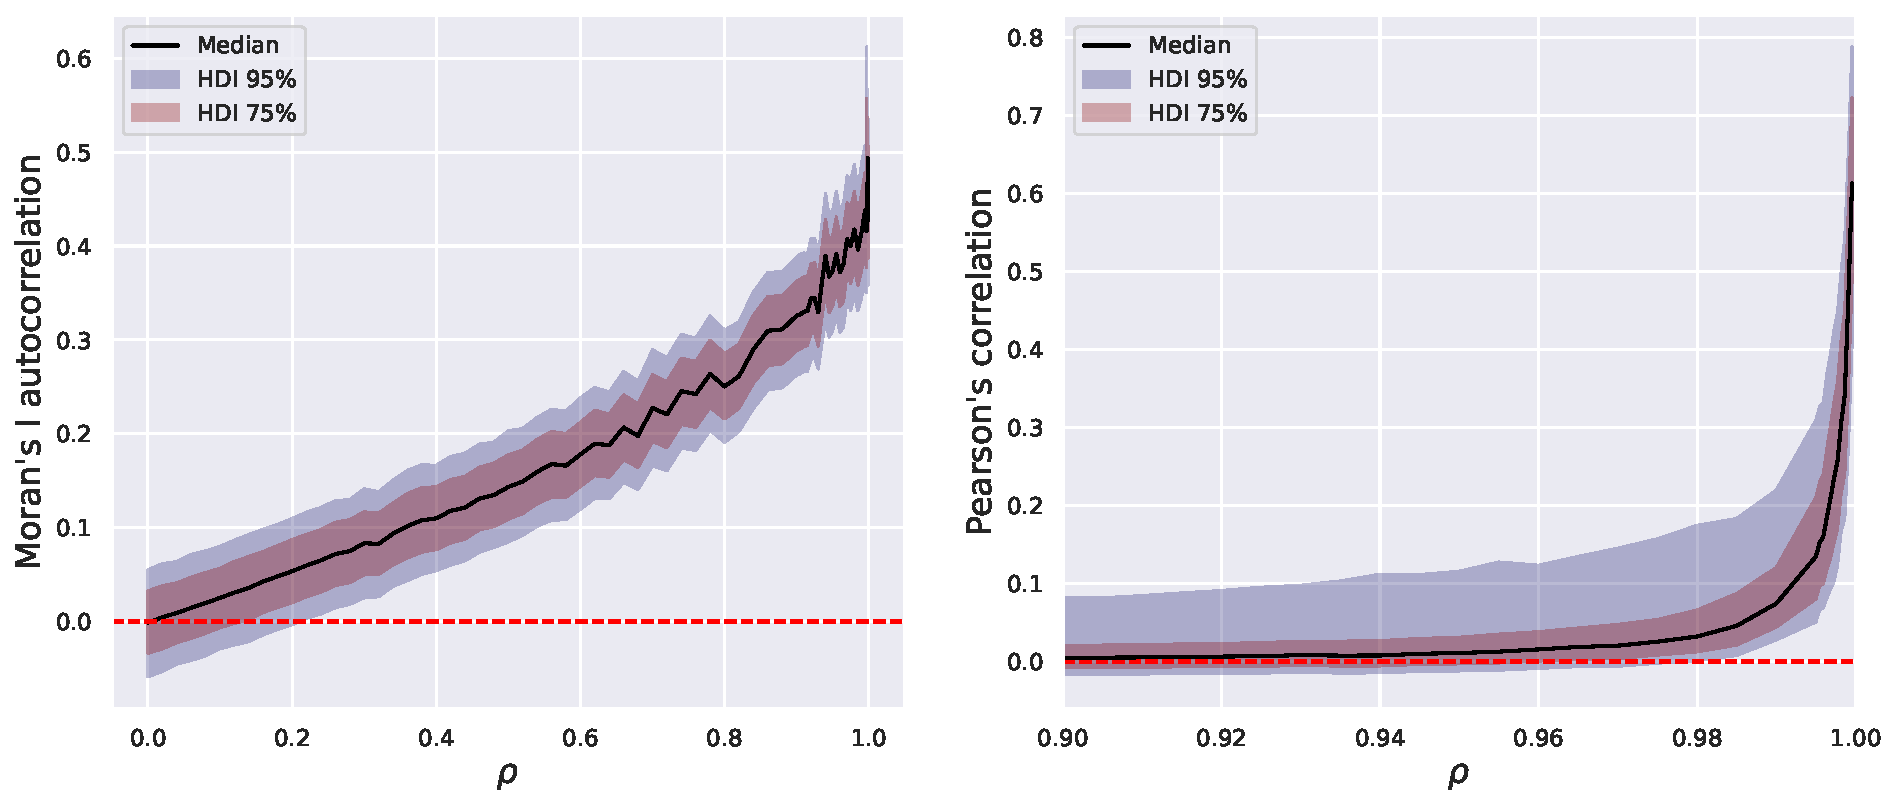
\includegraphics[width=12cm]{correlation-different-rho-values-car.pdf}
  \fonte{Prepared by the author (2021). The blue regions indicates the HDI
  95\%, while the red on is 
  the HDI 75\%. The black line denotes the median.}
\end{figure}

\begin{table}[htbp]
  \centering
  \caption{\label{tab:correlations-car-model}75\% Interval for Pearson's correlations among
  individuals for different values of $n$}
  \begin{tabular}{ccc}
  \hline
  \multirow{2}{*}{$n$} & \multicolumn{2}{c}{Interval 75\%} \\ \cline{2-3} 
   & Quartile 12.5\% & Quartile 87.5\% \\ \hline
  10 & 0.48 & 1.0 \\
  50 & 0.05 & 0.32 \\
  100 & 0.03 & 0.17 \\
  500 & -0.002 & 0.032 \\
  1000 & -0.007 & 0.02 \\ \hline
  \end{tabular}
  \fonte{Prepared by the author (2021).}
\end{table}

\section{Bayesian statistics}
\label{sec:bayesian_statistics}

We can represent our beliefs and information about unknown quantities 
through probabilities. There are two more common interpretations: 
frequentist and Bayesian. While the frequentists define
probability as the limit of a frequency in a large number of trials, the
Bayesians represent an individual's degree of belief in a statement that is
updated given new information. This philosophy allows assigning probabilities
to any event, even if a random process is not defined \cite{statisticat2016laplacesdemon}. 

In 1761, Reverend Thomas Bayes wrote for the first time the Bayes' formula
relating the probability of a parameter after observing the data with the
evidence (written through a likelihood function) and previous information
about the parameter. Pierre Simon Laplace rediscovered this formula in 1773
\cite{Robert2007}, and this theory became more common in the 19th century.
After some criticisms, a modern treatment considering Kolmogorov's
axiomatization of the theory of probabilities started after Jeffreys in 1939.
The recent development of new computational tools brought these ideas again.

Therefore, Bayesian inference is the process of inductive learning using
Bayes' rule, where inductive means that characteristics of a population are 
learned from a subset of it. We generally
express numerical characteristics of the population as a parameter $\theta$ which is
indirectly observed through numerical descriptions $y$ of the population. Both are
uncertain until the observation of a sample, when its information can decrease
our uncertainty about the population characteristics \cite[p. 1-2]{hoff2009first}.

The set of all possible outcomes $y$ forms the {\em sample space}
$\mathcal{Y}$, while the set of all possible parameters forms the {\em
parameter space} $\Theta$. Bayesian inference is composed by the following: 

\begin{alineas}
    \item {\em prior distribution:} A probability distribution defined over 
    $\Theta$ that quantifies our beliefs about $\theta$ before observing the data;
    \item {\em sampling model: } A probability distribution of the data generation process
    that express our belief that $y \in \mathcal{Y}$ is the outcome when
    $\theta \in \Theta$ is true. When it is seen as function of the parameter,
    it is called {\em likelihood function};
    \item {\em loss function:} Only in a decision theory framework, it
    measures the error of a estimative $\delta \in \Theta$ in comparison to
    $\theta$;
    \item {\em posterior distribution:} Once we get the data $y$, it
    represents our updated beliefs out the parameter conditioned All
    inferences are based on this probability distribution.
\end{alineas} 

Bayes' theorem establishes that when the sampling model is absolutely
continuous with respect to some measure $\nu$ with conditional density
$f_{Y\mid \theta}(y\mid\theta)$ and the prior distribution is a
well defined probability measure $\mu_{\theta}$, the posterior distribution
$\mu_{\theta|Y}(\cdot\mid y)$ is
absolutely continuous with respect to $\mu_{\theta}$ almost surely and its
Radon-Nikodym derivative is \cite[p. 16]{schervish2012theory}
\begin{equation}
  \label{eq:bayes-update-measure}
  \frac{d\mu_{\theta\mid Y}}{d\mu_{\theta}}(\theta|y) = \frac{f_{Y\mid \theta}(y\mid \theta)}{\int_{\Theta} f_{Y\mid\theta}(y|t)d\mu_{\theta}(t)}.  
\end{equation}

When the prior distribution is absolutely continuous with respect to the
Lebesgue measure, equation \eqref{eq:bayes-update-measure} resumes to 
\begin{equation}
  p(y|\theta) = \frac{f(y\mid \theta)\pi(\theta)}{\int_{\Theta} f(y\mid t)\pi(t) \, dt}.  
\end{equation}

Another important concept used thorough out the text is the following 

\begin{definition}
  \label{def:conjugate-family}
  Let $\mathcal{F}$ be a family of probability definitions parametrized by
  $\theta \in \Theta$. $\mathcal{F}$ is {\em conjugate} for a likelihood $f(y
  \mid \theta)$ when for every $\pi \in \mathcal{F}$, the posterior $p(y \mid
  \theta) \in \mathcal{F}$. The prior is called {\em conjugate prior} for the
  likelihood $p(y \mid \theta)$, and prior and posterior are {\em conjugate
  distributions}. 
\end{definition}

\section{Computational methods}
\label{sec:computational_methods}

Beyond the text, we use a state-of-art implementation of {\em Hamiltonian Monte
Carlo} (HMC) to sample from the posterior distribution of the parameters. HMC
is an advanced technique, and it is especially effective for hierarchical
models. In this section, we briefly describe the method and its diagnosis. 

HMC was developed in the late 1980s as a Hybrid MOnte Carlo to tackle
calculations in Lattice Quantum 

\subsection{Hamiltonian Monte Carlo}
\label{sec:hamiltonian-monte-carlo}

We follow \cite{betancourt2017conceptual}. This method was developed in the late 1980s as Hybrid Monte Carlo to tackle calculations in Lattice Quantum Chromodynamics. Instead of moving in the parameter space randomly with uninformed jumps, the direction from the vector field given by the gradients are used to trace out a trajectory through the *typical set*, the region which has significant contribution to the expectations. However, if only the gradient was used, the trajectory would pull towards the mode of the distribution, so more geometric constraints are needed. In order to a satellite rotate around the Earth, we have to endow ir with enough momentum to counteract the gravitational field, turning the system into a conservative one. 

First, we introduce auxiliary momentum parameters $p_n$ (lift) of the same dimension from the parameter space $\Omega \subseteq \mathbb{R}^D$. Then $q_n$ turns to $(q_n, p_n)$, with the use the joint probability distribution $\pi(q,p) = \pi(p\mid q)\pi(q)$. Particularly, we use 

$$
\pi(q,p) = e^{-H(q,p)}, 
$$

such that $H$ is the *Hamiltonian*. Note that $H(q,p) = -\log \pi(p\mid q) - \log \pi(q) =: K(p,q) + V(q)$. We call $K$ the kinetic energy, and $V$ the potential energy. The vector field is generated by Hamilton's equations, 

$$
\frac{dq}{dt} = \frac{\partial H}{\partial p} = \frac{\partial K}{\partial p}
$$
$$
\frac{dp}{dt} = -\frac{\partial H}{\partial q} = -\frac{\partial K}{\partial q} - \frac{d V}{d q}.
$$

Therefore, we are able to define the Hamiltonian flows $\phi_t : (p,q) \to
(p,q), \forall t \in \mathbb{R}$.

\subsubsection{Diagnostics}

The importance of diagnosing. The potential problems that it can show. 

\begin{itemize}
  \item Divergent transitions; 
  \item Transitions that hit the maximum tree depth; 
  \item Low E-BFMI values; 
  \item Low effective samples sizes; 
  \item $\hat{R} \not \in (0.95, 1.05)$.   
\end{itemize}

\subsection{Metropolis-within-Gibbs}

If this method is used. 